\section{Dart applications}

Creating a Flutter application can be done efficiently using the command line interface.
To start a new application, run the following command:
\begin{verbatim}
    flutter create app_name
\end{verbatim}
This command generates a directory structure containing essential subdirectories and files, some of which are automatically created for different platforms, while others are critical for development. 
The most important components include:
\begin{itemize}
    \item \texttt{lib} contains all your handwritten code, including the main Dart files that define your app.
    \item \texttt{pubspec.yaml} file: acts as the app's configuration file, managing external libraries and dependencies.
\end{itemize}

\paragraph*{Running the application}
Once the app is created, you can run it using:
\begin{verbatim}
    flutter run
\end{verbatim}
This command allows you to select the platform on which to run the app. 
If the required platforms are not available on your device, Flutter will emulate the target device for testing.

\subsection{Application structure}
The \texttt{lib} directory initially contains a \texttt{main.dart} file, which includes the following minimal code:
\begin{verbatim}
import 'package:flutter/material.dart';
    
void main() {
    runApp();
}
\end{verbatim}
You can choose between two styles: \texttt{material.dart} for material design or \texttt{cupertino.dart} for iOS-styled components.
The \texttt{runApp} function initializes the application, setting a widget as the root of the widget tree.
This tree typically consists of widgets like \texttt{Center} and \texttt{Text}, and Flutter ensures the root widget covers the entire screen.

\subsection{Functions}
n Dart, functions can have required positional parameters followed by optional named or optional positional parameters (but not both). 
Named parameters are optional unless explicitly marked as required. 
You can assign default values to both named and positional parameters using the \texttt{=} operator, but these must be compile-time constants. 
If no default value is specified, the default is \texttt{null}.

\paragraph*{Commas}
When writing Dart functions, methods, or constructors, always include a trailing comma in the parameter list. 
This practice helps Flutter's code formatter add proper line breaks and maintain code consistency.

\subsection{Widgets}
Flutter applications are composed entirely of widgets, which are the building blocks of the user interface. 
Below is an example of Flutter's material design structure:
\begin{figure}[H]
    \centering
    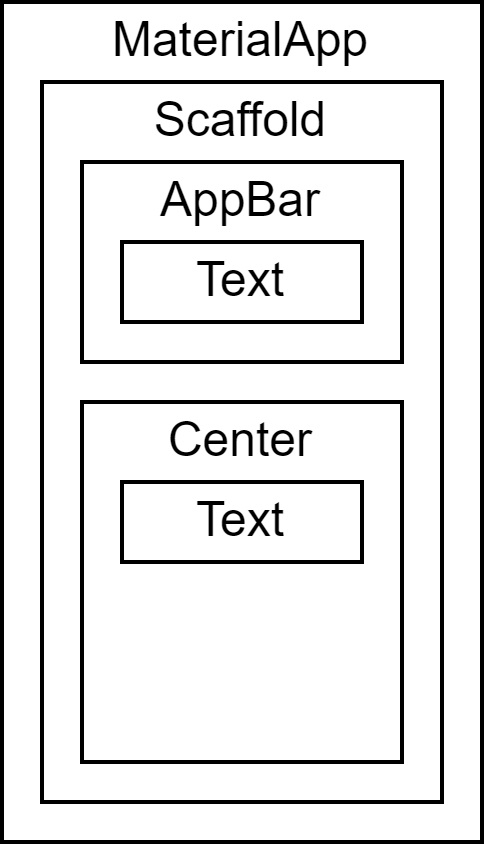
\includegraphics[width=0.25\linewidth]{images/material.png}
    \caption{Material structure}
\end{figure}
Key characteristics of widgets include:
\begin{itemize}
    \item \textit{Immutability}: widgets are immutable; once created, they cannot be changed. To modify their appearance or behavior, you must create a new widget.
    \item \textit{Composability}: widgets are composable, allowing developers to combine simpler widgets to create more complex interfaces.
    \item \textit{Descriptive nature}: widgets describe the UI, providing a visual representation of the interface components.
\end{itemize}

\paragraph*{Widget states}
Widgets can either be stateful or stateless:
\begin{itemize}
    \item \textit{Stateless widgets}: do not manage any internal state and are simple, static components of the UI.
    \item \textit{Stateful widgets}: maintain state that can change during the app's lifetime (e.g., the position of a slider). 
        Stateful widgets require two classes: one to extend \texttt{StatefulWidget} and another to manage the mutable state via the \texttt{State} object.
\end{itemize}
Stateful widgets use the \texttt{setState} method to notify Flutter that the state has changed, prompting the widget to be rebuilt and reflecting the updates in the UI.
State management is crucial for dynamic user interfaces.
When using the the \texttt{setState} method, Flutter knows that the state has changed and will re-render only the affected widgets, optimizing performance. 
Failing to call the \texttt{setState} when modifying state will leave the UI unchanged.

\paragraph*{Commond widgets}
The most common widgets are:
\begin{itemize}
    \item \textit{Flexible}: resizable widgets that adjust their size according to their \texttt{flex} and \texttt{fit} properties.
    \item \textit{Expanded}: forces a widget to take up all available space.
    \item \textit{SizedBox}: specifies a widget's dimensions or adds empty space.
    \item \textit{Spacer}: creates space between widgets using the \texttt{flex} property.
\end{itemize}

\subsection{Assets}
To include external assets in your project, you must declare them in \texttt{pubspec.yaml}. 
You can include all assets in a directory by specifying the directory name followed by a slash, e.g., \texttt{assets/}. 
For subdirectories, each must be listed separately.

Flutter's \texttt{AssetImage} class automatically selects the appropriate asset based on the device's pixel ratio, ensuring that the app displays optimally across different devices.

\subsection{Navigation}
Navigation in Flutter involves managing multiple screens (or routes). 
Routes represent screens, and you can navigate between them using:
\begin{itemize}
    \item \texttt{Navigator.push}: adds a new route to the stack.
    \item \texttt{Navigator.pop}: removes the current route from the stack, returning to the previous screen.
\end{itemize}
To pass data between routes, use \texttt{Navigator.pushNamed} and access arguments using \texttt{ModalRoute.of}.

\paragraph*{Asynchronous programming}
Dart uses \texttt{Future} objects to represent asynchronous operations. 
To define an asynchronous function, use the \texttt{async} keyword, and you can pause execution using the \texttt{await} keyword. 
This allows for handling asynchronous tasks such as network calls in a non-blocking manner.

\paragraph*{Adaptive design}
For responsive layouts, use widgets like \texttt{LayoutBuilder} and \texttt{MediaQuery}. 
\texttt{LayoutBuilder} returns layout constraints from the parent widget, while \texttt{MediaQuery} gives the size of the app window. 
This distinction helps in creating adaptive interfaces that work across various screen sizes.

\paragraph*{Advanced navigation}
For complex apps, especially web-based or multi-Navigator apps, using a \texttt{Router} allows for declarative navigation, integrating better with browser history and enabling advanced features like deep linking.
This structure ensures efficient state management, adaptive design, and smooth navigation throughout the app development lifecycle in Flutter.